\subsection{Glyph: \glyph{Unit of information}}
\label{sec:af:unitInfo}

When representing biological activities, it is often useful to illustrate the nature of the entity where the activity is originated, eg., whether the activity is from a macromolecule (protein or nucleic acid), or from a chemical compound.  The \SBGNAFLone \glyph{unit of information} is used in this situation to add such information to a glyph.  It represents the information in two ways.  First, different symbols are used to represent the nature of the entity where the activity is from.  These symbols are identical to the \glyph{entity pool node} symbols in SBGN \PDl.  Second, names of the entity (gene names, protein names) are usually provided as labels in the \glyph{unit of information} container.

\begin{glyphDescription}

\glyphSboTerm Not applicable.

\glyphContainer A unit of information is represented by containers of different shapes, depending on the nature of the entity where the biological activity is from. There are a total of five types of unit of information, as shown in \fig{af:unitInfo}.   Below is a summary of the five glyphs.

\begin{description}
\item[A.] macromolecule -- A unit of information of a macromolecule is represented by a rectangle with rounded corners, as illustrated in (A) of \fig{af:unitInfo}.  This container is used to decorate a biological activity that is originated from a macromolecule, such as a protein, a nucleic acid, or a complex sugar.

\item[B.] genetic -- A unit of information of a genetic entity is represented by a rectangle whose bottom half has rounded corners, as shown in (B) of  \fig{af:unitInfo}.

\item[C.] simple chemical -- A unit of information of a simple chemical is represented by a circular container, as shown in (C) of \fig{af:unitInfo}.

\item[D.] unspecified entity -- A unit of information of an unspecified entity is represented by an elliptic container, as shown in (D) of \fig{af:unitInfo}.  It is used to decorate a biological activity that is originated from an unspecified entity.

\item[E.] complex -- A unit of information of a complex is represented by an octagon as shown in (E) of \fig{af:unitInfo}.  It is used to decorate a biological activity that is originated from a complex.
\end{description}

The long side of the glyphs above (except for simple chemical) should be oriented parallel to the border of the \glyph{AN} being annotated by the \glyph{unit of information}. The center of the bounding box of a \glyph{state of information} should be located on the mid-line of the border of the \glyph{AN}.

\glyphLabel A \glyph{unit of information} is identified by a label placed in an unbordered box containing a string of characters. The characters can be distributed on several lines to improve readability, although this is not mandatory.  The label box must be attached to the center of the container. The label may spill outside of the container.  The label defines the information carried by the \glyph{unit of information}.

\glyphAux A \glyph{unit of information} does not carry any auxiliary items.

\end{glyphDescription}

\begin{figure}[H]
  \centering
  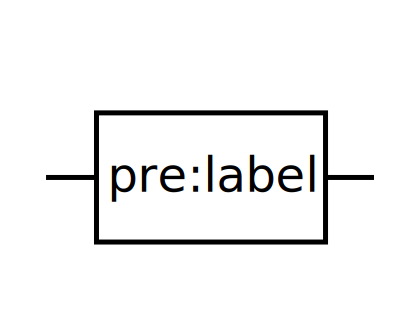
\includegraphics[scale = 0.2]{images/unitInformation}
  \caption{The \AF glyph for \glyph{unit of information}.}
  \label{fig:af:unitInfo}
\end{figure}

\fig{af:unitofinfo} shows examples units of information used on Activity Nodes to illustrate the properties of the entities that the activities are originated from.

\begin{figure}[H]
  \centering
  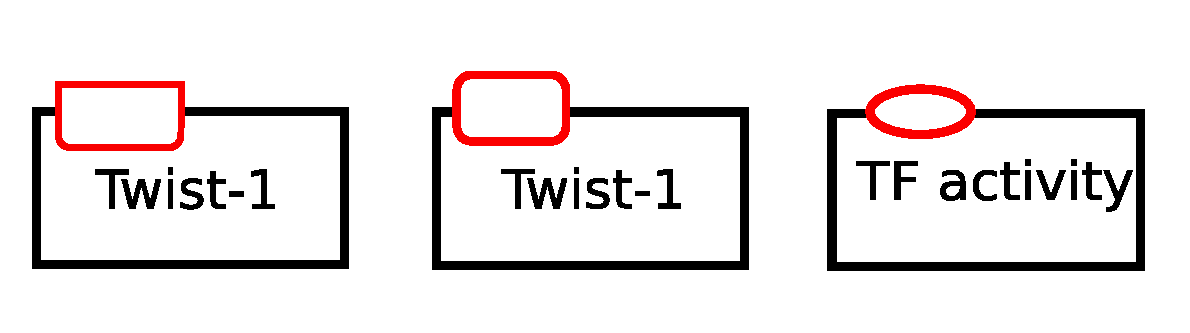
\includegraphics[scale = 0.5]{examples/unitofinformation}
  \caption{Examples of \glyph{unit of information} used on \glyph{biological activity node} to indicate that the activity is from a gene, a macromolecule, or unspecified.}
  \label{fig:af:unitofinfo}
\end{figure}